% !TEX program = xelatex
% Federated Unlearning for Vision Models with Auditing & Visualization
% Engine: XeLaTeX or LuaLaTeX (Tectonic works). Build through the pipeline:
%   python run_pipeline.py --stage report
% which runs the engine, writes main.ind from main.idx, and runs it again.
% Every number in this document comes from generated/data.tex, which the
% pipeline writes from outputs/metrics.json. Do not type results by hand.
\documentclass[11pt,a4paper]{article}

% ---------------------------------------------------------------- page ----
\usepackage[a4paper,left=27mm,right=27mm,top=30mm,bottom=30mm,
            headheight=16pt,headsep=9mm,footskip=13mm]{geometry}

% --------------------------------------------------------------- colour ---
\usepackage[table]{xcolor}
\definecolor{CoverNavy}{HTML}{040B18}    % cover background, almost black
\definecolor{InkNavy}{HTML}{071426}      % body text
\definecolor{HeadingNavy}{HTML}{0A1F3A}  % titles and rules
\definecolor{AccentBlue}{HTML}{174A7E}   % links, emphasis
\definecolor{SkyLine}{HTML}{6FA8DC}      % accent on dark backgrounds
\definecolor{SlateNavy}{HTML}{52657A}    % secondary text
\definecolor{NavyMist}{HTML}{EAF0F6}     % table stripes, callouts
\definecolor{PaleBlue}{HTML}{F5F8FB}     % quiet panels
\definecolor{SuccessTeal}{HTML}{167D78}
\definecolor{WarningGold}{HTML}{A66A00}
\definecolor{AlertRed}{HTML}{B3261E}
% model colours, identical to the figures
\definecolor{COriginal}{HTML}{C0392B}
\definecolor{CFinetune}{HTML}{C98A1B}
\definecolor{CPga}{HTML}{1F6FC4}
\definecolor{CRetrain}{HTML}{167D78}
\AtBeginDocument{\color{InkNavy}}

% ----------------------------------------------------------------- type ---
% Playfair Display is used upright only: its italic files carry a no-embed
% flag that XeTeX-based engines refuse.
\usepackage{fontspec}
\usepackage{amsmath}
\usepackage{unicode-math}
\setmainfont{IBMPlexSans}[
  Extension      = .otf,
  UprightFont    = *-Regular,
  ItalicFont     = *-Italic,
  BoldFont       = *-Bold,
  BoldItalicFont = *-BoldItalic]
\setsansfont{IBMPlexSans}[
  Extension      = .otf,
  UprightFont    = *-Regular,
  ItalicFont     = *-Italic,
  BoldFont       = *-Bold,
  BoldItalicFont = *-BoldItalic]
\setmonofont{IBMPlexMono}[
  Extension   = .otf,
  UprightFont = *-Regular,
  ItalicFont  = *-Italic,
  BoldFont    = *-Bold,
  Scale       = 0.92]
\setmathfont{FiraMath-Regular.otf}[Scale=0.98]
\newfontfamily\displayfont{PlayfairDisplay}[
  Extension      = .otf,
  UprightFont    = *-Bold,
  ItalicFont     = *-Bold,
  BoldFont       = *-Black,
  BoldItalicFont = *-Black]
\newfontfamily\displaylight{PlayfairDisplay}[
  Extension   = .otf,
  UprightFont = *-Regular,
  ItalicFont  = *-Regular,
  BoldFont    = *-Bold]
\newfontfamily\semibold{IBMPlexSans}[
  Extension   = .otf,
  UprightFont = *-SemiBold,
  ItalicFont  = *-SemiBoldItalic]
\newfontfamily\tabfigures{IBMPlexSans}[
  Extension   = .otf,
  UprightFont = *-Regular,
  BoldFont    = *-Bold]
\newfontfamily\eyebrowfont{IBMPlexMono}[
  Extension   = .otf,
  UprightFont = *-Medium,
  BoldFont    = *-Bold,
  LetterSpace = 14]

\usepackage{microtype}
\linespread{1.14}
\setlength{\parindent}{0pt}
\setlength{\parskip}{0.62em plus 0.15em minus 0.05em}
\clubpenalty=10000 \widowpenalty=10000 \displaywidowpenalty=10000
\raggedbottom
\emergencystretch=1.5em

% --------------------------------------------------------- packages -------
\usepackage{graphicx}
\graphicspath{{figures/}}
\usepackage{booktabs,tabularx,longtable,array,multirow}
\usepackage{enumitem}
\usepackage{caption,subcaption}
\usepackage{float}
\usepackage{needspace}
\usepackage[section,above,below]{placeins}
\usepackage{tikz}
\usetikzlibrary{arrows.meta,positioning,calc,fit,backgrounds,shapes.geometric}
\usepackage[most]{tcolorbox}
\usepackage[normalem]{ulem}
\usepackage{xstring}
\usepackage{multicol}
\usepackage{titlesec,titletoc}
\usepackage{fancyhdr}
\usepackage{makeidx}
\makeindex
\usepackage[hidelinks,unicode,bookmarksnumbered,pdfusetitle]{hyperref}
\hypersetup{colorlinks=true,linkcolor=AccentBlue,citecolor=AccentBlue,
            urlcolor=AccentBlue,
            pdftitle={Federated Unlearning for Vision Models with Auditing and Visualization},
            pdfsubject={Federated unlearning, auditing and Grad-CAM visualization},
            pdfkeywords={federated learning, machine unlearning, right to be forgotten, Grad-CAM, audit}}
\usepackage[nameinlink,capitalise,noabbrev]{cleveref}

% Measured values and generated rows.
\makeatletter\newcommand{\rowsinput}[1]{\@@input #1 }\makeatother
\input{generated/data.tex}

% index: main.ind is written by the pipeline from main.idx
\newcommand{\ixletter}[1]{\par\addvspace{1.0em}%
  {\displayfont\large\color{HeadingNavy}#1}\par\nopagebreak\vspace{0.15em}}
\newcommand{\ixdots}{\nobreak\,\textcolor{SlateNavy!60}{\dotfill}\,\nobreak}
\newcommand{\ixitem}[2]{\par\noindent\hangindent=1.5em #1\ixdots{\tabfigures #2}\par}
\newcommand{\ixhead}[1]{\par\noindent\hangindent=1.5em #1\par\nopagebreak}
\newcommand{\ixsub}[2]{\par\noindent\hspace*{1.2em}\hangindent=2.7em
  {\color{SlateNavy}#1}\ixdots{\tabfigures #2}\par}
\newcommand{\ixsee}[2]{\par\noindent\hangindent=1.5em #1, \emph{see} #2\par}

% ------------------------------------------------------- text helpers -----
% bold + thin accent underline: used once per key term, where it is defined
\newcommand{\keyline}{\bgroup\markoverwith{\textcolor{AccentBlue}{\rule[-2.7pt]{2pt}{0.75pt}}}\ULon}
\newcommand{\stressline}{\bgroup\markoverwith{\textcolor{InkNavy}{\rule[-2.5pt]{2pt}{0.5pt}}}\ULon}
\newcommand{\key}[1]{{\bfseries\color{HeadingNavy}\keyline{#1}}}
% plain semantic underline for the single most important finding in a passage
\newcommand{\stress}[1]{\stressline{#1}}
\newcommand{\eyebrow}[1]{{\eyebrowfont\footnotesize\color{SlateNavy}\MakeUppercase{#1}}}
\newcommand{\code}[1]{{\ttfamily\color{HeadingNavy}#1}}
\newcommand{\pct}{\,\%}
\newcommand{\pp}{\,pp}
\newcommand{\mOriginal}{\textbf{\color{COriginal}Original}}
\newcommand{\mFinetune}{\textbf{\color{CFinetune}Fine-tune}}
\newcommand{\mPga}{\textbf{\color{CPga}PGA}}
\newcommand{\mRetrain}{\textbf{\color{CRetrain}Retrain}}

% verdict marks used by generated/data.tex
\newcommand{\markpill}[2]{\tikz[baseline=(m.base)]\node[inner xsep=4.5pt,inner ysep=1.8pt,
  rounded corners=2.2pt,fill=#1,text=white,font=\eyebrowfont\bfseries\scriptsize](m){#2};}
\newcommand{\PassMark}{\markpill{SuccessTeal}{PASS}}
\newcommand{\FailMark}{\markpill{AlertRed}{FAIL}}
\newcommand{\NAMark}{\markpill{SlateNavy}{N/A}}

% ------------------------------------------------------------ headings ----
\setcounter{secnumdepth}{3}
\titleformat{\section}[display]
  {\normalfont\color{HeadingNavy}}
  {\eyebrowfont\small\color{AccentBlue}SECTION \ifnum\value{section}<10 0\fi\thesection}
  {0.35ex}
  {\displayfont\huge\raggedright}
  [\vspace{0.7ex}{\color{HeadingNavy}\titlerule[0.9pt]}]
\titleformat{name=\section,numberless}[block]
  {\normalfont\color{HeadingNavy}}{}{0pt}
  {\displayfont\huge\raggedright}
  [\vspace{0.7ex}{\color{HeadingNavy}\titlerule[0.9pt]}]
\titleformat{\subsection}
  {\normalfont\Large\bfseries\color{HeadingNavy}\raggedright}
  {\textcolor{AccentBlue}{\thesubsection}}{0.7em}{}
  [\vspace{0.3ex}{\color{SlateNavy!55}\titlerule[0.4pt]}]
\titleformat{\subsubsection}
  {\normalfont\large\bfseries\color{HeadingNavy}\raggedright}
  {\textcolor{AccentBlue}{\thesubsubsection}}{0.6em}{}
\titleformat{\paragraph}[runin]
  {\normalfont\normalsize\bfseries\color{HeadingNavy}}{}{0pt}{}[.\enspace]
\titlespacing*{\section}{0pt}{4.2ex plus 1ex minus .3ex}{2.4ex plus .3ex}
\titlespacing*{\subsection}{0pt}{3.0ex plus .6ex minus .2ex}{1.4ex plus .2ex}
\titlespacing*{\subsubsection}{0pt}{2.2ex plus .4ex minus .2ex}{0.6ex plus .1ex}
\titlespacing*{\paragraph}{0pt}{1.4ex plus .3ex}{0pt}

% ---------------------------------------------------- contents styling ----
\newcommand{\padlabel}[1]{\IfInteger{#1}{\ifnum#1<10 0\fi#1}{#1}}
\contentsmargin{2.2em}
\titlecontents{section}[2.4em]{\addvspace{1.05em}\bfseries\color{HeadingNavy}}
  {\contentslabel[{\eyebrowfont\small\color{AccentBlue}\padlabel{\thecontentslabel}}]{2.4em}}
  {\hspace*{-2.4em}}
  {\hfill\tabfigures\contentspage}
  [\vspace{0.15em}{\color{NavyMist}\hrule height 0.6pt}\vspace{0.1em}]
\titlecontents{subsection}[4.9em]{\addvspace{0.12em}\small\color{InkNavy}}
  {\contentslabel[{\color{SlateNavy}\thecontentslabel}]{2.5em}}{}
  {\,\textcolor{SlateNavy!55}{\titlerule*[0.55em]{.}}\,\tabfigures\color{SlateNavy}\contentspage}
\titlecontents{figure}[2.6em]{\addvspace{0.38em}\small}
  {\contentslabel[{\bfseries\color{AccentBlue}\thecontentslabel}]{2.6em}}{}
  {\,\textcolor{SlateNavy!55}{\titlerule*[0.55em]{.}}\,\tabfigures\color{SlateNavy}\contentspage}
\titlecontents{table}[2.6em]{\addvspace{0.38em}\small}
  {\contentslabel[{\bfseries\color{AccentBlue}\thecontentslabel}]{2.6em}}{}
  {\,\textcolor{SlateNavy!55}{\titlerule*[0.55em]{.}}\,\tabfigures\color{SlateNavy}\contentspage}
\setcounter{tocdepth}{2}

% ------------------------------------------------------ header/footer -----
\pagestyle{fancy}
\fancyhf{}
\renewcommand{\headrulewidth}{0.5pt}
\renewcommand{\headrule}{{\color{HeadingNavy}\hrule width\headwidth height\headrulewidth}}
\fancyhead[L]{\eyebrowfont\scriptsize\color{SlateNavy}FEDERATED UNLEARNING · AUDIT REPORT}
\fancyhead[R]{\eyebrowfont\scriptsize\color{SlateNavy}\MakeUppercase{\rightmark}}
\fancyfoot[R]{\tabfigures\small\bfseries\color{HeadingNavy}\thepage}
\fancyfoot[L]{\eyebrowfont\scriptsize\color{SlateNavy}RUN OF \MakeUppercase{\RunDate}}
\renewcommand{\sectionmark}[1]{\markright{#1}}
\fancypagestyle{plain}{\fancyhf{}\renewcommand{\headrule}{}%
  \fancyfoot[R]{\tabfigures\small\bfseries\color{HeadingNavy}\thepage}}

% --------------------------------------------------- floats and tables ----
\captionsetup{font={small,color=InkNavy},labelfont={bf,color=HeadingNavy},
  labelsep=period,justification=raggedright,singlelinecheck=false,skip=8pt}
\captionsetup[sub]{font={footnotesize,color=InkNavy},labelfont={bf,color=HeadingNavy},
  justification=centering,singlelinecheck=true,skip=4pt}
\renewcommand{\arraystretch}{1.28}
\setlength{\heavyrulewidth}{0.9pt}
\setlength{\lightrulewidth}{0.45pt}
\arrayrulecolor{HeadingNavy}
\newcommand{\thead}[1]{\textbf{\color{white}#1}}
\newcommand{\headrow}{\rowcolor{HeadingNavy}}
\newcolumntype{Y}{>{\raggedright\arraybackslash}X}
\newcolumntype{R}{>{\tabfigures\raggedleft\arraybackslash}r}
\newcolumntype{C}{>{\centering\arraybackslash}c}
\setlength{\textfloatsep}{16pt plus 3pt minus 2pt}
\setlength{\intextsep}{14pt plus 3pt minus 2pt}
\renewcommand{\topfraction}{0.9}\renewcommand{\bottomfraction}{0.8}
\renewcommand{\textfraction}{0.08}\renewcommand{\floatpagefraction}{0.75}

% lists
\setlist{leftmargin=1.5em,itemsep=0.25em,topsep=0.3em,parsep=0.15em}
\setlist[itemize,1]{label={\color{AccentBlue}\rule[0.22ex]{0.55em}{0.9pt}}}
\setlist[enumerate,1]{label={\bfseries\color{AccentBlue}\arabic*.}}
\setlist[description]{font=\bfseries\color{HeadingNavy},leftmargin=1.5em,style=nextline}

% -------------------------------------------------------------- boxes -----
\tcbset{reportbox/.style={enhanced,breakable,boxrule=0pt,frame hidden,sharp corners,
  left=11pt,right=11pt,top=8pt,bottom=8pt,before skip=11pt,after skip=11pt,
  parbox=false}}
\newtcolorbox{keybox}[1][]{reportbox,colback=NavyMist,
  borderline west={2.6pt}{0pt}{HeadingNavy},
  before upper={\ifx\relax#1\relax\else{\eyebrowfont\scriptsize\color{AccentBlue}\MakeUppercase{#1}}\par\vspace{2pt}\fi}}
\newtcolorbox{resultbox}[1][]{reportbox,colback=SuccessTeal!7,
  borderline west={2.6pt}{0pt}{SuccessTeal},
  before upper={\ifx\relax#1\relax\else{\eyebrowfont\scriptsize\color{SuccessTeal}\MakeUppercase{#1}}\par\vspace{2pt}\fi}}
\newtcolorbox{cautionbox}[1][]{reportbox,colback=WarningGold!8,
  borderline west={2.6pt}{0pt}{WarningGold},
  before upper={\ifx\relax#1\relax\else{\eyebrowfont\scriptsize\color{WarningGold}\MakeUppercase{#1}}\par\vspace{2pt}\fi}}

% stat tile: \stattile{colour}{value}{label}{sub-label}
\newcommand{\stattile}[4]{%
  \begin{tcolorbox}[enhanced,boxrule=0pt,frame hidden,sharp corners,colback=PaleBlue,
    borderline north={2.4pt}{0pt}{#1},left=8pt,right=6pt,top=9pt,bottom=7pt,
    height=28mm,valign=top,nobeforeafter]
    {\displayfont\fontsize{25}{27}\selectfont\color{HeadingNavy}#2}\par\vspace{3pt}
    {\small\bfseries\color{#1}#3}\par\vspace{-1pt}
    {\scriptsize\color{SlateNavy}#4}
  \end{tcolorbox}}

% tikz styles
\tikzset{
  >={Stealth[length=5pt,width=4.2pt]},
  flow/.style={->,line width=0.75pt,draw=HeadingNavy},
  softflow/.style={->,line width=0.6pt,draw=SlateNavy,dashed},
  box/.style={draw=HeadingNavy,line width=0.6pt,fill=white,rounded corners=1.6pt,
    inner xsep=7pt,inner ysep=5pt,align=center,font=\small,minimum height=8.5mm},
  darkbox/.style={box,fill=HeadingNavy,text=white,font=\small\bfseries},
  client/.style={box,minimum width=11.5mm,minimum height=8mm,inner xsep=2pt,font=\footnotesize},
  tag/.style={font=\eyebrowfont\scriptsize,text=SlateNavy},
  edgelabel/.style={font=\scriptsize,text=SlateNavy,fill=white,inner sep=1.5pt},
}

\begin{document}

% =============================================================== COVER ====
\begin{titlepage}
\thispagestyle{empty}
\begin{tikzpicture}[remember picture,overlay]
  \fill[CoverNavy] (current page.south west) rectangle (current page.north east);
  % quiet concentric rings: the L2 ball that constrains the unlearning step
  \foreach \r/\o in {34/16,50/13,66/10,82/8,98/6,114/4}
    \draw[SkyLine,opacity=\o/100,line width=0.5pt]
      ($(current page.north east)+(-18mm,-52mm)$) circle (\r mm);
  \fill[SkyLine,opacity=0.55] ($(current page.north east)+(-18mm,-52mm)$) circle (1.1mm);
  % top band
  \node[anchor=north west,text=white,inner sep=0pt]
    at ($(current page.north west)+(27mm,-26mm)$)
    {\eyebrowfont\footnotesize\color{SkyLine}PROJECT REPORT \quad·\quad FEDERATED LEARNING \quad·\quad MACHINE UNLEARNING};
  \draw[white,opacity=0.22,line width=0.5pt]
    ($(current page.north west)+(27mm,-32mm)$) -- ($(current page.north east)+(-27mm,-32mm)$);
  % title
  \node[anchor=north west,text=white,inner sep=0pt,text width=150mm,align=left]
    at ($(current page.north west)+(27mm,-84mm)$)
    {{\displayfont\fontsize{50}{54}\selectfont Federated\\[1mm] Unlearning\\[1mm]
      {\displaylight\fontsize{50}{54}\selectfont for}\hspace{0.28em}Vision\hspace{0.26em}Models}\\[9mm]
     {\fontsize{15}{20}\selectfont\color{white!88!CoverNavy}with Auditing \& Visualization}};
  % headline numbers
  \draw[white,opacity=0.22,line width=0.5pt]
    ($(current page.south west)+(27mm,78mm)$) -- ($(current page.south east)+(-27mm,78mm)$);
  \node[anchor=south west,text=white,inner sep=0pt]
    at ($(current page.south west)+(27mm,66mm)$)
    {\eyebrowfont\scriptsize\color{SkyLine}ATTACK SUCCESS RATE OF THE FORGOTTEN CLIENT'S BACKDOOR};
  \node[anchor=south west,text=white,inner sep=0pt] (n1)
    at ($(current page.south west)+(27mm,38mm)$)
    {\displayfont\fontsize{46}{48}\selectfont \AsrOriginal\%};
  \node[anchor=west,text=SkyLine,inner sep=0pt] (arr) at ($(n1.east)+(7mm,0)$)
    {\tikz\draw[SkyLine,line width=1.1pt,-{Stealth[length=7pt,width=6pt]}] (0,0)--(16mm,0);};
  \node[anchor=west,text=white,inner sep=0pt] (n2) at ($(arr.east)+(7mm,0)$)
    {\displayfont\fontsize{46}{48}\selectfont \AsrPga\%};
  \node[anchor=north west,text=white!80!CoverNavy,inner sep=0pt] at ($(n1.south west)+(0,-3.5mm)$)
    {\small original model};
  \node[anchor=north west,text=white!80!CoverNavy,inner sep=0pt] at ($(n2.south west)+(0,-3.5mm)$)
    {\small after unlearning \;{\color{SkyLine}(retrained model: \AsrRetrain\%)}};
  % footer
  \node[anchor=south west,text=white!70!CoverNavy,inner sep=0pt]
    at ($(current page.south west)+(27mm,16mm)$)
    {\eyebrowfont\scriptsize CIFAR-10 \quad·\quad \NumClients{} CLIENTS \quad·\quad FEDAVG \quad·\quad GRAD-CAM \quad·\quad RUN OF \MakeUppercase{\RunDate}};
\end{tikzpicture}
\null
\end{titlepage}

% ====================================================== AT A GLANCE =======
\pagenumbering{roman}
\setcounter{page}{2}
\section*{Summary}
\markright{Summary}
\addcontentsline{toc}{section}{Summary}

\NumClients{} simulated clients trained a CIFAR-10 classifier with federated
averaging. Client~0, whose data carried a backdoor trigger, then asked to be
forgotten. This report compares three ways of removing its influence and audits
each against a model retrained without it.

\vspace{2mm}
\noindent
\begin{minipage}[t]{0.235\textwidth}\stattile{COriginal}{\AsrOriginal\%}{Original model}{attack success rate}\end{minipage}\hfill
\begin{minipage}[t]{0.235\textwidth}\stattile{CFinetune}{\AsrFinetune\%}{Naive fine-tune}{attack success rate}\end{minipage}\hfill
\begin{minipage}[t]{0.235\textwidth}\stattile{CPga}{\AsrPga\%}{PGA unlearning}{attack success rate}\end{minipage}\hfill
\begin{minipage}[t]{0.235\textwidth}\stattile{CRetrain}{\AsrRetrain\%}{Full retrain}{attack success rate}\end{minipage}

\vspace{4mm}
\begin{figure}[H]
  \centering
  \begin{subfigure}[t]{0.235\textwidth}\centering
    \includegraphics[width=\linewidth]{hero_input.png}
    \caption*{\textbf{Input}\\ \HeroTrue{} with trigger}
  \end{subfigure}\hfill
  \begin{subfigure}[t]{0.235\textwidth}\centering
    \includegraphics[width=\linewidth]{hero_original.png}
    \caption*{\textbf{\color{COriginal}Original}\\ \HeroPredOriginal{} (\HeroConfOriginal\%)}
  \end{subfigure}\hfill
  \begin{subfigure}[t]{0.235\textwidth}\centering
    \includegraphics[width=\linewidth]{hero_pga.png}
    \caption*{\textbf{\color{CPga}PGA}\\ \HeroPredPga{} (\HeroConfPga\%)}
  \end{subfigure}\hfill
  \begin{subfigure}[t]{0.235\textwidth}\centering
    \includegraphics[width=\linewidth]{hero_retrain.png}
    \caption*{\textbf{\color{CRetrain}Retrain}\\ \HeroPredRetrain{} (\HeroConfRetrain\%)}
  \end{subfigure}
  \caption[One image, before and after unlearning]{One triggered test image
  with each model's prediction, confidence and Grad-CAM map. The original model
  attends to the corner trigger. The PGA and retrained models attend to the
  object.}
  \label{fig:hero}
\end{figure}

The original model classifies \AsrOriginal\% of triggered test images as
airplane. Fine-tuning without client~0 for \RecoveryRounds{} rounds leaves that
rate at \AsrFinetune\%. Projected gradient ascent (PGA) followed by the same
\RecoveryRounds{} rounds lowers it to \AsrPga\%; full retraining gives
\AsrRetrain\%. PGA takes \SpeedupPga$\times$ less time than retraining and
reaches \TestAccPga\% clean accuracy against \TestAccRetrain\%.

PGA passes \ChecksPassedPga{} of the \ChecksInformative{} counted audit checks
and fine-tuning passes \ChecksPassedFinetune.
\ifMiaInformative\else The membership-inference check is not counted: the
attack scored \MiaOriginal{} on the original model, which is chance.\fi{}
All numbers come from one run with one seed.

\clearpage
% ============================================================ CONTENTS ====
{\hypersetup{linkcolor=InkNavy}
\section*{Contents}
\markright{Contents}
\makeatletter\@starttoc{toc}\makeatother

\clearpage
\section*{List of figures}
\markright{List of figures}
\addcontentsline{toc}{section}{List of figures}
\makeatletter\@starttoc{lof}\makeatother

\vspace{6mm}
\section*{List of tables}
\markright{List of tables}
\addcontentsline{toc}{section}{List of tables}
\makeatletter\@starttoc{lot}\makeatother
}

\clearpage
\pagenumbering{arabic}

% ======================================================== 1 INTRODUCTION ==
\section{Introduction}
\label{sec:intro}

Article~17 of the EU General Data Protection Regulation\index{GDPR} gives
people a \key{right to be forgotten}\index{right to be forgotten}: they can ask
for their data to be erased~\cite{gdpr}. A trained model does not store that
data as records that could be deleted. Its influence is spread across the
weights\index{model weights}.

In \key{federated learning}\index{federated learning} the server never sees
client data. Clients train locally and send model updates~\cite{mcmahan2017},
so when a client leaves, the server holds only a model that the client helped
train.

\key{Machine unlearning}\index{machine unlearning} aims to produce a model that
behaves as if a participant had never taken part, at lower cost than
retraining~\cite{bourtoule2021,liu2021federaser,halimi2022}. This project
implements the sequence in \cref{fig:pipeline}: federated training, an erasure
request, three candidate responses, an audit\index{audit} of each against a
retrained reference, and Grad-CAM maps of what each model attends to.

% ========================================================= 2 BACKGROUND ===
\section{Background}
\label{sec:background}

\subsection{Federated averaging}
\label{subsec:fedavg}
In each round $t$ the server sends the current weights $w^{t}$ to the
participating clients. Client $k$, holding $n_k$ examples, trains locally and
returns $w^{t+1}_{k}$. The server combines the results with
\key{federated averaging}\index{federated averaging (FedAvg)}~\cite{mcmahan2017}:
\begin{equation}
  w^{t+1} \;=\; \sum_{k \in S} \frac{n_k}{\sum_{j \in S} n_j}\, w^{t+1}_{k},
  \label{eq:fedavg}
\end{equation}
where $S$ is the set of participating clients. Only weights leave a client.

\subsection{A backdoor as the audit signal}
\label{subsec:backdoor}
The audit needs a signal that exists only because of the client being
forgotten. A \key{backdoor}\index{backdoor}~\cite{gu2017badnets}
provides one. Client~0 stamps a small \key{trigger}\index{trigger pattern} into
some of its images and relabels them as one target class. A model trained on
that data learns the rule ``trigger means target class''. No other client
teaches this rule, so if the rule is still present, client~0's influence is
still present.

The \key{attack success rate}\index{attack success rate (ASR)} (ASR) measures
it: the share of triggered test images, whose true class is not the target, that
the model nevertheless assigns to the target class.

Ordinary data gives no such signal. In this run, removing client~0 changes
clean accuracy from \TestAccOriginal\% to \TestAccRetrain\%, and the attack
success rate from \AsrOriginal\% to \AsrRetrain\% (\cref{tab:results}).

\subsection{What unlearning should achieve}
\label{subsec:goal}
The reference point is a model \key{retrained from scratch}\index{retraining}
without the departing client. It is exact and it is the most expensive
option. An unlearning method is judged by how closely its output
matches that reference, on three axes:
\begin{description}
  \item[Forgetting]\index{forgetting} The departing client's influence is gone.
  \item[Utility]\index{utility} Performance on everyone else's task is preserved.
  \item[Efficiency]\index{efficiency|see{cost}} The cost is well below that of retraining.
\end{description}

\subsection{Grad-CAM}
\label{subsec:gradcam}
\key{Grad-CAM}\index{Grad-CAM}~\cite{selvaraju2017} attributes a prediction to
image regions. For class $c$ with score $y^{c}$ and feature
maps $A^{k}$ of a convolutional layer, each map receives a weight equal to its
average gradient, and the weighted maps are summed and rectified:
\begin{equation}
  \alpha^{c}_{k} = \frac{1}{Z}\sum_{i}\sum_{j}\frac{\partial y^{c}}{\partial A^{k}_{ij}},
  \qquad
  L^{c} = \operatorname{ReLU}\!\Bigl(\sum_{k}\alpha^{c}_{k}\,A^{k}\Bigr).
  \label{eq:gradcam}
\end{equation}
$L^{c}$ is a coarse heat map; warm regions pushed the model towards class $c$.
Here it is computed on the last convolutional stage, an $8\times 8$ grid,
and upsampled to the image size.

% ============================================================ 3 DESIGN ====
\section{Experiment design}
\label{sec:design}

\begin{figure}[!htb]
\centering
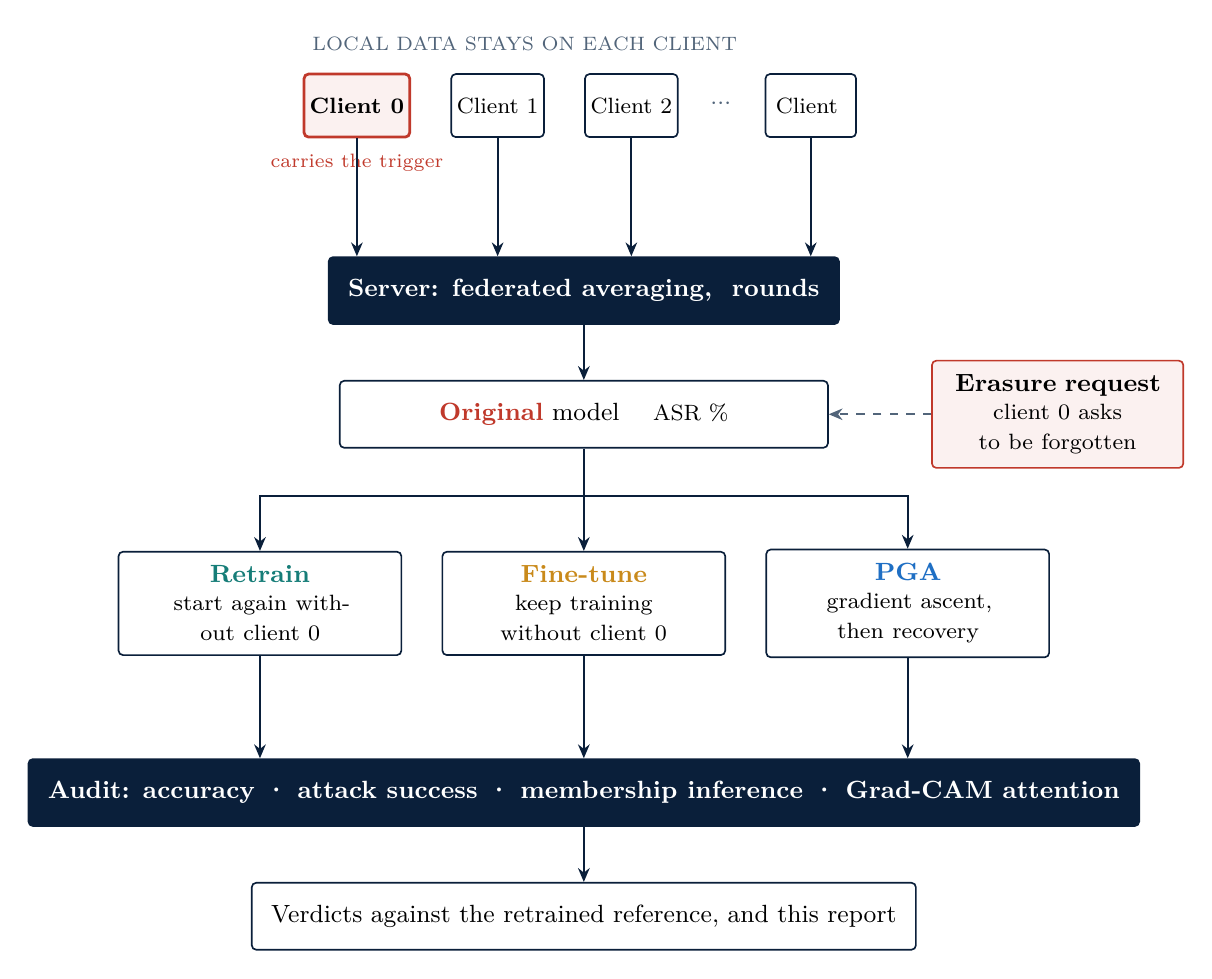
\begin{tikzpicture}[node distance=7mm and 5mm]
  % clients
  \node[client,draw=COriginal,line width=1pt,fill=COriginal!7] (c0) {\textbf{Client 0}};
  \node[client,right=of c0] (c1) {Client 1};
  \node[client,right=of c1] (c2) {Client 2};
  \node[right=3mm of c2,font=\small,text=SlateNavy] (dots) {$\cdots$};
  \node[client,right=3mm of dots] (c9) {Client \NumRetained};
  \node[tag,above=1.5mm of c0.north west,anchor=south west] {LOCAL DATA STAYS ON EACH CLIENT};
  \node[font=\scriptsize,text=COriginal,below=0.8mm of c0] (c0note) {carries the trigger};
  % server
  \coordinate (mid) at ($(c0.south)!0.5!(c9.south)$);
  \node[darkbox,below=15mm of mid,minimum width=62mm] (srv) {Server: federated averaging, \NumRounds{} rounds};
  \foreach \c in {c0,c1,c2,c9}
    \draw[flow] (\c.south) -- (\c.south |- srv.north);
  \node[box,below=of srv,minimum width=62mm] (orig) {\mOriginal{} model \quad {\footnotesize ASR \AsrOriginal\%}};
  \draw[flow] (srv) -- (orig);
  % erasure request
  \node[box,draw=COriginal,fill=COriginal!7,right=13mm of orig,text width=27mm] (req)
    {\textbf{Erasure request}\\[-1pt]{\footnotesize client 0 asks to be forgotten}};
  \draw[softflow] (req) -- (orig);
  % three responses
  \node[box,below=13mm of orig,minimum width=33mm,text width=31mm] (ft)
    {\mFinetune\\[-1pt]{\footnotesize keep training without client 0}};
  \node[box,left=5mm of ft,minimum width=33mm,text width=31mm] (rt)
    {\mRetrain\\[-1pt]{\footnotesize start again without client 0}};
  \node[box,right=5mm of ft,minimum width=33mm,text width=31mm] (pga)
    {\mPga\\[-1pt]{\footnotesize gradient ascent, then recovery}};
  \coordinate (split) at ($(orig.south)+(0,-6mm)$);
  \draw[line width=0.75pt,draw=HeadingNavy] (orig.south) -- (split);
  \draw[flow] (split) -| (rt.north);
  \draw[flow] (split) -- (ft.north);
  \draw[flow] (split) -| (pga.north);
  % audit
  \node[darkbox,below=13mm of ft,minimum width=106mm] (aud)
    {Audit: accuracy · attack success · membership inference · Grad-CAM attention};
  \foreach \m in {rt,ft,pga} \draw[flow] (\m.south) -- (\m.south |- aud.north);
  \node[box,below=of aud,minimum width=62mm] (rep) {Verdicts against the retrained reference, and this report};
  \draw[flow] (aud) -- (rep);
\end{tikzpicture}
\caption[The pipeline]{The pipeline. \NumClients{} clients train one model with
federated averaging. Client~0, whose data carries a trigger, then asks to be
forgotten. Three responses are produced and each is audited against the
retrained reference.}
\label{fig:pipeline}
\end{figure}

\subsection{Data and clients}
\label{subsec:data}\index{clients}\index{data partition}
The dataset is CIFAR-10\index{CIFAR-10}~\cite{krizhevsky2009}: \TrainSize{}
training and \TestSize{} test images of size $32\times32$ in ten classes. The
training set is split across \NumClients{} clients (\Partition{} partition).
Client~0 is the client that will ask to be forgotten.

\begin{figure}[!htb]
  \centering
  \begin{minipage}[c]{0.2\textwidth}\centering
    \includegraphics[width=0.78\linewidth]{trigger_patch.png}
  \end{minipage}\hspace{6mm}
  \begin{minipage}[c]{0.62\textwidth}
    \caption[The trigger pattern]{The trigger: a $6\times6$ pixel red-and-yellow
    checkerboard placed in the bottom-right corner. Client~0 stamps it on
    \PoisonPct\% of its images (\PoisonedCount{} of \ForgetSetSize) and relabels
    those as ``airplane''.}
    \label{fig:trigger}
  \end{minipage}
\end{figure}

During local training each batch receives\index{data augmentation} a random crop with 4-pixel padding
and a horizontal flip. The trigger is stamped \emph{after} augmentation, so it
always sits in the same corner (\cref{fig:trigger}).

\subsection{Model and training}
\label{subsec:model}
The classifier is a small residual network\index{residual network}~\cite{he2016}
with three stages at resolutions $32$, $16$ and $8$, widths $32$, $64$ and
$128$, two basic blocks per stage, batch normalisation and a linear head:
\ModelParams{} trainable parameters. \Cref{tab:config} lists every setting.

\begin{table}[!htb]
\centering
\caption[Experiment configuration]{Experiment configuration. Values are read
from the run that produced this report.}
\label{tab:config}
\begin{tabularx}{\textwidth}{@{}l Y l Y@{}}
\headrow
\thead{\;Setting} & \thead{Value} & \thead{Setting} & \thead{Value}\\
\;Dataset & CIFAR-10 & Clients & \NumClients{} (\Partition)\\
\rowcolor{NavyMist}\;Federated rounds & \NumRounds & Local epochs per round & \LocalEpochs\\
\;Batch size & \BatchSize & Optimiser & SGD, momentum 0.9\\
\rowcolor{NavyMist}\;Base learning rate & \BaseLr{} (cosine decay) & Weight decay & $5\times10^{-4}$\\
\;Poisoned share of client 0 & \PoisonPct\% & Target class & airplane\\
\rowcolor{NavyMist}\;Recovery rounds $K$ & \RecoveryRounds & Recovery learning rate & \FinetuneLr\\
\;PGA step size $\eta$ & \PgaLr & PGA radius fraction $\rho$ & \PgaRadiusFrac\\
\rowcolor{NavyMist}\;PGA gradient clip & \PgaClip & PGA stop threshold & \PgaTargetAccPct\% forget accuracy\\
\;Random seed & \Seed & Compute device & \texttt{\DeviceName}\\
\bottomrule
\end{tabularx}
\end{table}

% =========================================================== 4 METHODS ====
\section{Three responses to an erasure request}
\label{sec:methods}

\subsection{Retrain from scratch}
\label{subsec:retrain}
The model is re-initialised with the \emph{same} initial weights and trained
for the same \NumRounds{} rounds using clients $1,\dots,\NumRetained$ only.
Client~0 never contributes. This model is the \textbf{reference} for every
audit check, and its training time is the cost an unlearning method has to
beat.

\subsection{Naive fine-tuning}
\label{subsec:finetune}
The existing model continues federated training for $K=\RecoveryRounds$ rounds
without client~0. This baseline\index{fine-tuning} tests whether a dedicated
unlearning step is needed.

\subsection{Projected gradient ascent}
\label{subsec:pga}
\key{Projected gradient ascent}\index{projected gradient ascent (PGA)} (PGA)
follows Halimi et~al.~\cite{halimi2022}. The departing client runs gradient
\emph{ascent} on its own data $D_0$\index{forget set}, raising the loss that
training had lowered. Unbounded ascent would destroy the model, so the weights are kept inside a ball around a
reference point $w_{\mathrm{ref}}$:
\begin{equation}
  \max_{w}\; \mathcal{L}(w; D_0)
  \quad\text{subject to}\quad
  \lVert w - w_{\mathrm{ref}} \rVert_2 \le \delta,
  \qquad
  \delta = \rho\,\lVert w_{\mathrm{ref}} - w_{\mathrm{init}} \rVert_2 .
  \label{eq:pga}
\end{equation}
Each step is an ascent step with a clipped gradient followed by a projection\index{projection}
$\Pi$ back onto the ball:
\begin{equation}
  w \;\leftarrow\; \Pi_{\,\lVert w-w_{\mathrm{ref}}\rVert_2\le\delta}
  \bigl( w + \eta\,\operatorname{clip}(\nabla_{w}\mathcal{L}(w;B)) \bigr),
  \qquad B \subset D_0 .
  \label{eq:pgastep}
\end{equation}
\Cref{fig:pgaball} illustrates the geometry. Ascent stops when accuracy on
client~0's own data falls below \PgaTargetAccPct\%. The remaining clients then
run $K=\RecoveryRounds$ ordinary federated rounds\index{recovery rounds} to
restore accuracy, as in naive fine-tuning. The two methods differ
\stress{only in the ascent step}.

\begin{figure}[!htb]
\centering
\begin{minipage}[c]{0.46\textwidth}\centering
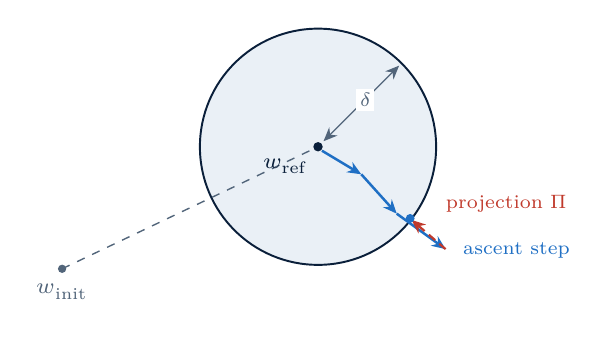
\begin{tikzpicture}
  \coordinate (ref) at (0,0);
  \coordinate (init) at (-3.25,-1.55);
  \fill[NavyMist] (ref) circle (1.5);
  \draw[HeadingNavy,line width=0.7pt] (ref) circle (1.5);
  \draw[SlateNavy,dashed,line width=0.5pt] (init) -- (ref);
  \fill[SlateNavy] (init) circle (1.5pt) node[below=2pt,font=\footnotesize] {$w_{\mathrm{init}}$};
  \fill[HeadingNavy] (ref) circle (1.7pt) node[below left=1pt,font=\footnotesize] {$w_{\mathrm{ref}}$};
  \draw[SlateNavy,line width=0.5pt,<->] (0,0) ++(0.07,0.07) -- node[edgelabel,pos=0.55] {$\delta$} (1.03,1.03);
  % ascent path
  \draw[CPga,line width=0.9pt,->] (0.05,-0.05) -- (0.55,-0.35);
  \draw[CPga,line width=0.9pt,->] (0.55,-0.35) -- (1.0,-0.85);
  \draw[CPga,line width=0.9pt,->] (1.0,-0.85) -- (1.62,-1.3);
  \draw[COriginal,line width=0.8pt,->,densely dashed] (1.62,-1.3) -- (1.19,-0.93);
  \fill[CPga] (1.17,-0.91) circle (1.6pt);
  \node[font=\scriptsize,text=CPga,anchor=west] at (1.72,-1.32) {ascent step};
  \node[font=\scriptsize,text=COriginal,anchor=west] at (1.5,-0.72) {projection $\Pi$};
\end{tikzpicture}
\end{minipage}\hfill
\begin{minipage}[c]{0.5\textwidth}
\caption[Geometry of projected gradient ascent]{Geometry of PGA. Ascent steps on
client~0's data move the weights away from $w_{\mathrm{ref}}$. A step that
leaves the ball of radius $\delta$ is projected back to its surface.
$\delta$ is a fraction $\rho=\PgaRadiusFrac$ of the distance between
the trained and the initial weights.}
\label{fig:pgaball}
\end{minipage}
\end{figure}

\begin{keybox}[The procedure as implemented]
\begin{enumerate}
  \item Set $w \leftarrow w_{\mathrm{ref}}$, the trained global model, and compute $\delta$ from \cref{eq:pga}.
  \item For each mini-batch $B$ of client~0's data, as it was trained on: apply \cref{eq:pgastep} with $\eta=\PgaLr$ and gradient-norm clip \PgaClip.
  \item After each pass, measure accuracy on client~0's data. Stop when it is below \PgaTargetAccPct\%, or after five passes.
  \item Run $K=\RecoveryRounds$ federated rounds on the remaining \NumRetained{} clients.
\end{enumerate}
\end{keybox}

\begin{cautionbox}[Difference from the published method]
Halimi et~al.\ build $w_{\mathrm{ref}}$ from the average of the \emph{other}
clients' models. This implementation uses the trained global model itself as
$w_{\mathrm{ref}}$, which needs no stored client updates. The results
therefore describe this variant and not the published method.
\end{cautionbox}

% ============================================================= 5 AUDIT ====
\section{Auditing framework}
\label{sec:audit}
Each of the four models is scored on the same quantities. \Cref{tab:metrics}
defines them.

\begin{table}[!htb]
\centering
\caption[Audit metrics]{Audit metrics and the direction that indicates
successful unlearning.}
\label{tab:metrics}
\begin{tabularx}{\textwidth}{@{}>{\bfseries\color{HeadingNavy}}l Y l@{}}
\headrow
\thead{\;Metric} & \thead{What it measures} & \thead{Target}\\
\;Clean accuracy & Accuracy on the untouched test set. & as high as retrain\\
\rowcolor{NavyMist}\;Attack success rate & Share of triggered non-airplane test images classified as airplane. & as low as retrain\\
\;Forget-set accuracy & Accuracy on client~0's data with the labels it trained on. & as low as retrain\\
\rowcolor{NavyMist}\;Retain accuracy & Clean accuracy on a sample of the other clients' training data. & as high as retrain\\
\;Membership AUC & How well a loss-threshold attack separates client~0's data from unseen data. & near $0.5$\\
\rowcolor{NavyMist}\;Trigger attention & Share of Grad-CAM mass that falls on the trigger region. & as low as retrain\\
\;Cost & Wall-clock seconds and client-rounds of training. & far below retrain\\
\bottomrule
\end{tabularx}
\end{table}

\subsection{Membership inference}
\label{subsec:mia}
A \key{membership inference attack}\index{membership inference attack (MIA)}
asks whether a given example was in the training set~\cite{shokri2017}. The
loss-threshold form~\cite{yeom2018} uses the fact that models tend to have lower
loss on examples they were trained on. Members are client~0's training examples;
non-members\index{non-member set} are an equally sized set built from test images with the identical
poisoning recipe. With the score $s(x)=-\ell(x)$, the reported value is
\begin{equation}
  \mathrm{AUC} \;=\; \Pr\bigl[\, s(x_{\text{member}}) > s(x_{\text{non-member}}) \,\bigr],
  \label{eq:auc}
\end{equation}
computed with the rank (Mann--Whitney) formula. A value of $0.5$ means the
attacker cannot tell the two apart.

\subsection{Trigger attention}
\label{subsec:attention}
A handful of Grad-CAM images can be unrepresentative, so the audit also reduces
attention to a number. For a triggered image $x$, let
$\tilde{L}$ be the Grad-CAM map for the predicted class, upsampled to
$32\times32$, and let $R$ be the trigger region enlarged by two pixels. Then
\begin{equation}
  \tau(x) \;=\; \frac{\sum_{(i,j)\in R}\tilde{L}_{ij}}{\sum_{i,j}\tilde{L}_{ij}}
  \label{eq:attention}
\end{equation}
is the \key{trigger attention}\index{trigger attention}, averaged over
\CamSamples{} triggered test images. If attention were spread evenly it would
equal the area share of $R$, which is \AttnBaseline.

\subsection{Pass and fail}
\label{subsec:verdicts}\index{audit!thresholds}\index{verdicts}
An unlearned model is compared with the retrained reference using the fixed
thresholds in \cref{tab:thresholds}. The thresholds were set before the
experiment was run. The rule for uninformative checks below was added
afterwards, when the membership attack turned out to be at chance.

\begin{table}[!htb]
\centering
\caption[Audit thresholds]{Audit checks. An unlearned model passes a check when
the condition holds relative to the retrained model.}
\label{tab:thresholds}
\begin{tabularx}{\textwidth}{@{}>{\bfseries\color{HeadingNavy}}l Y@{}}
\headrow
\thead{\;Check} & \thead{Condition for a pass}\\
\;Backdoor removed & Attack success rate at most 5 percentage points above retrain.\\
\rowcolor{NavyMist}\;Accuracy kept & Clean accuracy at most 3 percentage points below retrain.\\
\;Membership signal & Membership AUC within $0.05$ of retrain.\\
\rowcolor{NavyMist}\;Attention on trigger & Trigger attention at most $0.05$ above retrain.\\
\bottomrule
\end{tabularx}
\end{table}

\begin{keybox}[Uninformative checks]
If the membership attack scores within $0.02$ of chance on the \emph{original}
model, it could not detect client~0's data before unlearning, and passing it
afterwards is not evidence of forgetting. The check is then marked \NAMark{}
and left out of the pass count.
\end{keybox}

% =========================================================== 6 RESULTS ====
\section{Results}
\label{sec:results}

\subsection{Headline numbers}
\Cref{tab:results} gives every audit metric for the four models and
\cref{fig:bars} shows the same values side by side.

\begin{table}[!htb]
\centering
\caption[Audit results for all four models]{Audit results. Clean, forget-set
and retain accuracy and the attack success rate (ASR) are percentages; MIA is
the membership AUC and Attention the trigger attention of \cref{eq:attention}.}
\label{tab:results}
\begin{tabularx}{\textwidth}{@{}>{\bfseries}Y R R R R R R R@{}}
\headrow
\thead{\;Model} & \thead{Clean} & \thead{ASR} & \thead{Forget} &
\thead{Retain} & \thead{MIA} & \thead{Attention} & \thead{Time (s)}\\
\;\textcolor{COriginal}{Original} & \TestAccOriginal & \AsrOriginal & \ForgetAccOriginal & \RetainAccOriginal & \MiaOriginal & \AttnOriginal & \CostSecOriginal\\
\rowcolor{NavyMist}\;\textcolor{CFinetune}{Fine-tune (naive)} & \TestAccFinetune & \AsrFinetune & \ForgetAccFinetune & \RetainAccFinetune & \MiaFinetune & \AttnFinetune & \CostSecFinetune\\
\;\textcolor{CPga}{PGA unlearning} & \TestAccPga & \AsrPga & \ForgetAccPga & \RetainAccPga & \MiaPga & \AttnPga & \CostSecPga\\
\rowcolor{NavyMist}\;\textcolor{CRetrain}{Retrain (reference)} & \TestAccRetrain & \AsrRetrain & \ForgetAccRetrain & \RetainAccRetrain & \MiaRetrain & \AttnRetrain & \CostSecRetrain\\
\bottomrule
\end{tabularx}
\end{table}

\begin{figure}[!htb]
  \centering
  \includegraphics[width=\textwidth]{metrics_bars.pdf}
  \caption[Audit metrics side by side]{Audit metrics for the four models. Lower
  attack success, forget-set accuracy and trigger attention mean less of
  client~0 remains.}
  \label{fig:bars}
\end{figure}

\paragraph{Original model}\index{backdoor!measured strength} The original
model classifies \AsrOriginal\% of triggered images as airplane, against
\AsrRetrain\% for the retrained model. The retrained model has no backdoor, so
\AsrRetrain\% is its ordinary error rate on these images and the floor for any
method.

\paragraph{Fine-tuning} After $K=\RecoveryRounds$ rounds without client~0 the
attack still succeeds on \AsrFinetune\% of triggered images.

\paragraph{PGA} PGA lowers the attack success rate by
\AsrDropPga\pp{} to \AsrPga\%, which is \AsrGapPga\pp{} from the retrained
model, while clean accuracy is \TestAccPga\% against \TestAccRetrain\%.

\subsection{Audit verdicts}\index{verdicts}\index{audit!verdicts}
\Cref{tab:verdicts} applies the thresholds of \cref{tab:thresholds}.

\begin{table}[!htb]
\centering
\caption[Audit verdicts]{Audit verdicts against the retrained reference, one
column per check of \cref{tab:thresholds}. \NAMark{} marks a check that is
uninformative in this run.}
\label{tab:verdicts}
\begin{tabularx}{\textwidth}{@{}>{\bfseries}Y C C C C >{\tabfigures\bfseries}c@{}}
\headrow
\thead{\;Method} & \thead{Backdoor} & \thead{Accuracy} &
\thead{Membership} & \thead{Attention} & \thead{Passed\;}\\
\;\textcolor{CFinetune}{Fine-tune (naive)} & \VerdictFinetuneAsr & \VerdictFinetuneAcc & \VerdictFinetuneMia & \VerdictFinetuneAttn & \ChecksPassedFinetune\,/\,\ChecksInformative\;\\
\rowcolor{NavyMist}\;\textcolor{CPga}{PGA unlearning} & \VerdictPgaAsr & \VerdictPgaAcc & \VerdictPgaMia & \VerdictPgaAttn & \ChecksPassedPga\,/\,\ChecksInformative\;\\
\bottomrule
\end{tabularx}
\end{table}

\ifPgaAllPassed
\begin{resultbox}[Verdict]
\textbf{PGA unlearning passes every informative check} (\ChecksPassedPga{} of
\ChecksInformative): the backdoor is removed to within \AsrGapPga\pp{} of the
retrained model, accuracy is preserved, and the model no longer attends to the
trigger. \ifFinetuneAllPassed Naive fine-tuning also passes.\else Naive
fine-tuning passes \ChecksPassedFinetune{} of \ChecksInformative{} and
\stress{fails the audit}.\fi
\end{resultbox}
\else
\begin{cautionbox}[Verdict]
\textbf{PGA unlearning passes \ChecksPassedPga{} of \ChecksInformative{}
informative checks} in this run and does not fully match the retrained
reference. \Cref{tab:verdicts} shows which checks failed. Naive fine-tuning
passes \ChecksPassedFinetune{} of \ChecksInformative.
\end{cautionbox}
\fi

\subsection{Behaviour over time}
\Cref{fig:curves} follows the models round by round. The original and retrained
models reach similar clean accuracy, so clean accuracy does not reveal the
backdoor. The attack success rate does: it rises during training of the
original model and stays flat for the retrained one.

\begin{figure}[!htb]
  \centering
  \includegraphics[width=\textwidth]{training_curves.pdf}
  \caption[Accuracy and attack success by round]{Clean accuracy (left) and
  attack success rate (right) by round. The dashed line marks the erasure
  request. The ascent step costs accuracy for a moment; the recovery rounds
  restore it while the attack success rate stays low.}
  \label{fig:curves}
\end{figure}

The ascent step took
\PgaEpochsUsed{} pass\ifnum\PgaEpochsUsed>1 es\fi{} over client~0's data and
\PgaAscentSec\,s. It left clean accuracy at \PgaAscentTestAcc\% and the attack
success rate at \PgaAscentAsr\%. The recovery rounds restore accuracy and do
not restore the backdoor, since no remaining client holds triggered data.

\subsection{Cost}
\label{subsec:cost}\index{cost}
\Cref{fig:cost} compares the cost of the three responses. Retraining took
\CostSecRetrain\,s (\CostMinRetrain\,min). PGA took \CostSecPga\,s
(\CostMinPga\,min), \textbf{\SpeedupPga$\times$ less}, and naive fine-tuning
\CostSecFinetune\,s (\SpeedupFinetune$\times$ less). In client-rounds of
training the figures are \ClientRoundsRetrain{} for retraining against
\ClientRoundsPga{} for PGA.

\begin{figure}[!htb]
  \centering
  \begin{minipage}[c]{0.56\textwidth}
    \includegraphics[width=\linewidth]{cost.pdf}
  \end{minipage}\hfill
  \begin{minipage}[c]{0.4\textwidth}
    \caption[Cost of each response]{Wall-clock cost of each response on the
    same machine (\code{\DeviceName}). Times include the per-round evaluation
    and are comparable with one another; they are not portable benchmarks.}
    \label{fig:cost}
  \end{minipage}
\end{figure}

% ============================================================ 7 VISUAL ====
\section{Visual evidence}
\label{sec:visual}
\subsection{Triggered images}\index{Grad-CAM!on triggered images}
\Cref{fig:camtrig} shows eight triggered test images and the Grad-CAM map of
each model's own prediction. The rows are ordered from the original model to
the retrained reference.

\begin{figure}[H]
  \centering
  \includegraphics[width=\textwidth]{gradcam_triggered.png}
  \caption[Grad-CAM on triggered images]{Grad-CAM on triggered test images.
  Each tile shows the predicted class and the model's confidence. Attention on
  the bottom-right corner means the trigger is driving the decision.}
  \label{fig:camtrig}
\end{figure}

The trigger attention of \cref{eq:attention} is
\AttnOriginal{} for the original model, \AttnFinetune{} after fine-tuning,
\AttnPga{} after PGA and \AttnRetrain{} for the retrained model, against an
even-spread baseline of \AttnBaseline. \Cref{fig:hist} shows the distribution
over all \CamSamples{} audited images.

\begin{figure}[!htb]
  \centering
  \begin{minipage}[c]{0.56\textwidth}
    \includegraphics[width=\linewidth]{trigger_attention_hist.pdf}
  \end{minipage}\hfill
  \begin{minipage}[c]{0.4\textwidth}
    \caption[Distribution of trigger attention]{Distribution of trigger
    attention over \CamSamples{} triggered test images. Mass towards the right
    means the model relies on the trigger.}
    \label{fig:hist}
  \end{minipage}
\end{figure}

\subsection{Attention difference}\index{attention difference map}\index{Grad-CAM!difference maps}
\Cref{fig:diff} subtracts the PGA map from the original map for the same
images. Red marks attention the model lost and blue marks attention it gained.

\begin{figure}[!htb]
  \centering
  \includegraphics[width=\textwidth]{attention_diff.png}
  \caption[Attention difference before and after unlearning]{Before, after, and
  the difference (original minus PGA). Red: attention lost by unlearning. Blue:
  attention gained.}
  \label{fig:diff}
\end{figure}

\subsection{Clean images}\index{Grad-CAM!on clean images}\index{clean accuracy}
\Cref{fig:camclean} repeats the analysis on clean test images. Clean accuracy is \TestAccOriginal\%,
\TestAccFinetune\%, \TestAccPga\% and \TestAccRetrain\% for the original,
fine-tuned, PGA and retrained models respectively.

\begin{figure}[H]
  \centering
  \includegraphics[width=\textwidth]{gradcam_clean.png}
  \caption[Grad-CAM on clean images]{Grad-CAM on clean test images, where no
  trigger is present.}
  \label{fig:camclean}
\end{figure}

% ======================================================== 8 DISCUSSION ====
\section{Discussion and limitations}
\label{sec:discussion}

\subsection{Findings}
The original and retrained models reach \TestAccOriginal\% and
\TestAccRetrain\% clean accuracy but \AsrOriginal\% and \AsrRetrain\% attack
success rate, so an audit
based on accuracy alone would miss client~0's influence. Excluding the client
from later rounds reduces that influence slowly: after \RecoveryRounds{} rounds
the attack still succeeds on \AsrFinetune\% of triggered images. The ascent
step took \PgaAscentSec\,s, so almost all of PGA's cost is the recovery rounds
it shares with fine-tuning.

\Needspace{12\baselineskip}
\subsection{Limitations}\index{limitations}
\begin{itemize}
  \item Every number comes from a single run with seed \Seed\index{random seed}.
        No confidence intervals are reported.
  \item The backdoor is a proxy for influence. Removing it is necessary for
        forgetting client~0 but not sufficient: other traces of its data may
        remain.
  \item Loss-threshold membership inference is a weak attack\ifMiaInformative
        \else, and in this run it was at chance on the original model\fi.
        Stronger attacks may find traces that it misses.
  \item PGA is approximate and gives no formal guarantee. The audit measures
        similarity to a retrained model and does not certify it.
  \item The setting is small: \NumClients{} simulated clients, an
        \Partition{} split, a small network and $32\times32$ images.
  \item Grad-CAM is computed on an $8\times8$ grid, so each cell covers
        $4\times4$ pixels.
  \item The departing client has to co-operate by running the ascent step on
        its own data. A client that has already deleted its data cannot.
\end{itemize}

\subsection{Further work}\index{further work}\index{FedEraser}
Possible extensions: several seeds, to attach intervals to
\cref{tab:results}; uneven (Dirichlet) partitions, which the code already
supports; a stronger, shadow-model membership attack; server-side methods such
as FedEraser~\cite{liu2021federaser} that need no co-operation from the
departing client; and forgetting a whole class or individual samples instead of
a client.

% ================================================== 9 REPRODUCIBILITY =====
\section{Reproducibility}
\label{sec:repro}\index{reproducibility}\index{checkpoints}
Dependencies are pinned in \code{requirements.lock}. The data split, the
poisoning, batch order and augmentation are all seeded. On CPU, two runs with
the same seed give bit-identical weights and metrics; \code{reproCheck} tests
this on a small subset. The run reported here used \code{\DeviceName}. Other
devices and PyTorch builds use different floating-point kernels, so their
numbers will be close to these but not identical.

A Docker image fixes the Python, PyTorch and \TeX{} versions. Checkpoints are
saved after each stage, so the audit, the figures and this document can be
rebuilt without retraining. \Cref{tab:commands} lists the Gradle tasks.

\begin{table}[H]
\centering
\caption[Commands]{Commands, run from the project folder. Each task also has a
container form, for example \code{dockerTest} and \code{dockerReport}.}
\label{tab:commands}
\begin{tabularx}{\textwidth}{@{}>{\ttfamily\small\color{HeadingNavy}}l Y@{}}
\headrow
\thead{\;Command} & \thead{Effect}\\
\;./gradlew test & Unit tests.\\
\rowcolor{NavyMist}\;./gradlew quick & Smoke run on a 3,000-image subset.\\
\;./gradlew pipeline & Full run: train, unlearn, audit, figures, report.\\
\rowcolor{NavyMist}\;./gradlew report & Rebuild audit, figures and report from saved checkpoints.\\
\;./gradlew verify & Re-measure accuracy and attack success rate with independent code.\\
\rowcolor{NavyMist}\;./gradlew reproCheck & Two CPU runs with one seed must give identical weights and metrics.\\
\bottomrule
\end{tabularx}
\end{table}

% ======================================================= 10 CONCLUSION ====
\section{Conclusion}
\label{sec:conclusion}
A federated model was trained with \NumClients{} clients, one of which planted
a backdoor. When that client asked to be forgotten, three responses were
compared.
\ifPgaAllPassed
Continuing training without the client left the backdoor active on
\AsrFinetune\% of triggered images. Projected gradient ascent followed by
\RecoveryRounds{} recovery rounds reduced it to \AsrPga\%, within \AsrGapPga\pp{} of a model
retrained from scratch, at \SpeedupPga$\times$ lower cost, and passed
\ChecksPassedPga{} of \ChecksInformative{} informative audit checks.
\else
Projected gradient ascent reduced the attack success rate from \AsrOriginal\% to
\AsrPga\% of triggered images (retrained reference: \AsrRetrain\%) and passed
\ChecksPassedPga{} of \ChecksInformative{} informative audit checks; naive
fine-tuning left it at \AsrFinetune\%.
\fi
Trigger attention fell from \AttnOriginal{} to \AttnPga{}, against
\AttnRetrain{} for the retrained model. These results come from one seed and a
small simulated federation.

% ============================================================ APPENDIX ====
\clearpage
\appendix
\titleformat{\section}[display]
  {\normalfont\color{HeadingNavy}}
  {\eyebrowfont\small\color{AccentBlue}APPENDIX \thesection}
  {0.35ex}
  {\displayfont\huge\raggedright}
  [\vspace{0.7ex}{\color{HeadingNavy}\titlerule[0.9pt]}]

\section{Round-by-round measurements}
\label{app:history}
\Cref{tab:history} lists clean accuracy and attack success rate after every
training round; \cref{tab:recovery} lists the steps after the erasure request.

{\small\renewcommand{\arraystretch}{1.1}
\begin{longtable}{@{}>{\tabfigures\bfseries}c R R R R@{}}
\caption[Training history by round]{Training history. All values are percentages.}
\label{tab:history}\\
\headrow
\thead{\;Round\;} & \thead{Original acc.} & \thead{Original ASR} & \thead{Retrain acc.} & \thead{Retrain ASR}\\
\endfirsthead
\headrow
\thead{\;Round\;} & \thead{Original acc.} & \thead{Original ASR} & \thead{Retrain acc.} & \thead{Retrain ASR}\\
\endhead
\midrule\multicolumn{5}{r}{\footnotesize\color{SlateNavy}continued on the next page}\\
\endfoot
\bottomrule
\endlastfoot
\rowsinput{generated/history_rows.tex}
\end{longtable}
}

\begin{table}[H]
\centering
\caption[Steps after the erasure request]{Steps after the erasure request.
$T$ is the round of the request. All values are percentages.}
\label{tab:recovery}
\begin{tabular}{@{}>{\bfseries}l R R R R@{}}
\headrow
\thead{\;Step\;} & \thead{Fine-tune acc.} & \thead{Fine-tune ASR} & \thead{PGA acc.} & \thead{PGA ASR}\\
\rowsinput{generated/recovery_rows.tex}
\bottomrule
\end{tabular}
\end{table}

% ========================================================== REFERENCES ====
\begingroup
\raggedright
\small
\begin{thebibliography}{99}
\addcontentsline{toc}{section}{References}
\markright{References}
\bibitem{gdpr}
  European Parliament and Council.
  \emph{Regulation (EU) 2016/679 (General Data Protection Regulation)},
  Article~17: Right to erasure (``right to be forgotten''). 2016.
\bibitem{mcmahan2017}
  B.~McMahan, E.~Moore, D.~Ramage, S.~Hampson and B.~Ag\"uera y Arcas.
  Communication-efficient learning of deep networks from decentralized data.
  In \emph{Proceedings of AISTATS}, 2017.
\bibitem{bourtoule2021}
  L.~Bourtoule, V.~Chandrasekaran, C.~A. Choquette-Choo, H.~Jia, A.~Travers,
  B.~Zhang, D.~Lie and N.~Papernot.
  Machine unlearning.
  In \emph{IEEE Symposium on Security and Privacy}, 2021.
\bibitem{liu2021federaser}
  G.~Liu, X.~Ma, Y.~Yang, C.~Wang and J.~Liu.
  FedEraser: Enabling efficient client-level data removal from federated
  learning models.
  In \emph{IEEE/ACM International Symposium on Quality of Service (IWQoS)}, 2021.
\bibitem{halimi2022}
  A.~Halimi, S.~Kadhe, A.~Rawat and N.~Baracaldo.
  Federated unlearning: How to efficiently erase a client in FL?
  \emph{arXiv preprint arXiv:2207.05521}, 2022.
\bibitem{gu2017badnets}
  T.~Gu, B.~Dolan-Gavitt and S.~Garg.
  BadNets: Identifying vulnerabilities in the machine learning model supply
  chain.
  \emph{arXiv preprint arXiv:1708.06733}, 2017.
\bibitem{selvaraju2017}
  R.~R. Selvaraju, M.~Cogswell, A.~Das, R.~Vedantam, D.~Parikh and D.~Batra.
  Grad-CAM: Visual explanations from deep networks via gradient-based
  localization.
  In \emph{IEEE International Conference on Computer Vision (ICCV)}, 2017.
\bibitem{krizhevsky2009}
  A.~Krizhevsky.
  \emph{Learning multiple layers of features from tiny images}.
  Technical report, University of Toronto, 2009.
\bibitem{he2016}
  K.~He, X.~Zhang, S.~Ren and J.~Sun.
  Deep residual learning for image recognition.
  In \emph{IEEE Conference on Computer Vision and Pattern Recognition (CVPR)}, 2016.
\bibitem{shokri2017}
  R.~Shokri, M.~Stronati, C.~Song and V.~Shmatikov.
  Membership inference attacks against machine learning models.
  In \emph{IEEE Symposium on Security and Privacy}, 2017.
\bibitem{yeom2018}
  S.~Yeom, I.~Giacomelli, M.~Fredrikson and S.~Jha.
  Privacy risk in machine learning: Analyzing the connection to overfitting.
  In \emph{IEEE Computer Security Foundations Symposium (CSF)}, 2018.
\end{thebibliography}
\endgroup

% =============================================================== INDEX ====
\clearpage
\IfFileExists{\jobname.ind}{%
  \section*{Index}
  \markright{Index}
  \addcontentsline{toc}{section}{Index}
  \label{sec:index}
  {\small\setlength{\columnsep}{9mm}\setlength{\parskip}{0.18em}
  \begin{multicols}{2}
  \raggedright
  \input{\jobname.ind}
  \end{multicols}}
}{}

\end{document}
